\section{Results}
In this section we will present and compare the results obtained with the two approaches. 
Some results obtained from a randomly piloted battleship are considered as baseline.

For both NEAT and GP, the evolution process stores at each run the best program generated with the
relative statistical results and plots in the 'runs' folder. In this way, it is
possible to launch the program later and observe through the game interface how the battleship behaves.


\subsection{NEAT}
The NEAT algorithm managed to evolve a ANN that can reach level 42 in the game with a
fitness of 1114 after about 160 generations. The ANN is represented in Fig. \ref{fig:NEAT_best}. As we can
see the network is quite simple, with a small number of nodes and connections: it has just 10
hidden nodes and 63 enabled connections (that are represented by the solid arrows).


In Fig. \ref{fig:NEAT_fitness}, we can observe that the best fitness increases significantly in just a few particular
generations, whereas the average fitness does not grow significantly and stays under 200.
With this fitness trend, we can also notice that the speciation decreases significantly after 20
generations due to the stagnation of a lot of species: after about 60 generations, 
just the 2 elitism species will survive as shown in Fig. \ref{fig:NEAT_speciation}.

A weak point of NEAT is that the generated ANN is not really interpretable and we cannot
understand why the network produces certain output values.

\begin{figure}[ht]
\centerline{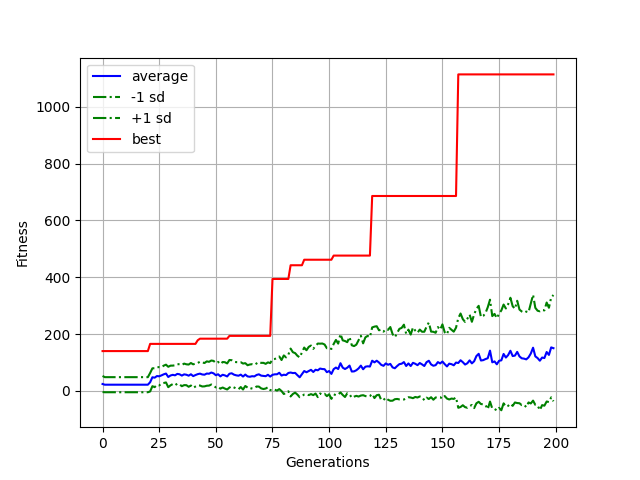
\includegraphics[scale=0.55]{NEAT_fitness.png}}
\caption{Fitness trend of the NEAT run that has generated the best ANN.}
\label{fig:NEAT_fitness}
\end{figure}


\begin{figure}[ht]
\centerline{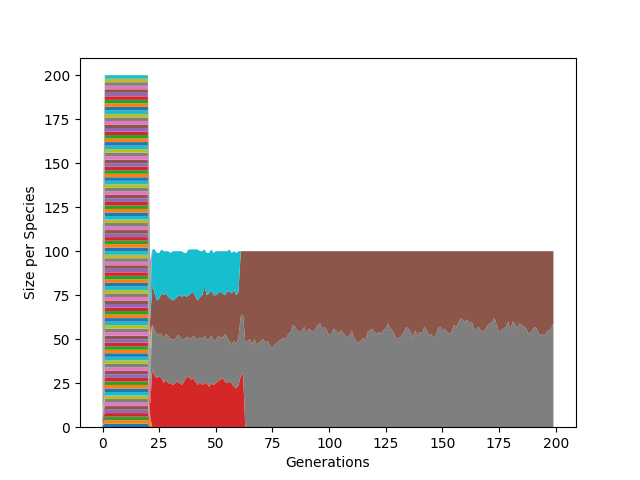
\includegraphics[scale=0.55]{NEAT_speciation.png}}
\caption{Speciation trend of the NEAT run that has generated the best ANN.}
\label{fig:NEAT_speciation}
\end{figure}


\subsection{GP}
The GP algorithm managed to evolve two tree-based programs that reach over 4000 fitness in the simulation.

The first program reaches level 151 in the
game with a fitness of 4061 during the evolution process and level 194 with a fitness of 5212
without limiting the number of frames. The tree of the program is represented in Fig. \ref{fig:GP_best1}. As
we can see the tree is quite complex, with 259 nodes and a depth of 10 (the maximum depth
allowed). In Fig. \ref{fig:GP_fitness1}, we can observe that the best fitness improves a lot in the first 60
generations reaching the frame threshold.

The second program reaches level 162 in the game with a fitness of 4342 during the evolution process and 
level 189 with a fitness of 5076 without limiting the number of frames. The tree of the program is 
represented in Fig. \ref{fig:GP_best2}. As we can see the tree is a bit less complex than the previous one, with 177 nodes 
and a depth of 10 (the maximum depth allowed). As shown in Fig. \ref{fig:GP_fitness2}, the best fitness improves significantly 
only after 100 generations, reaching the frame threshold.

In both cases, for the remaining generations, the best fitness trend increases slightly, probably also due 
to this limitation on the number of frames. The average fitness trend is smoother and follows the best trend 
with a similar increase, reaching about 3000 fitness with a large variance (over 1000).

A weak point of GP is that the generated tree is a bit complex and can be simplified a lot,
e.g. simplifying some "if\_then\_else" statements that have as condition pure boolean values as can be
seen in Fig. \ref{fig:GP_best}.

\begin{figure*}[t!]
    \centering
    \begin{subfigure}[b]{0.45\textwidth}
        \centering
        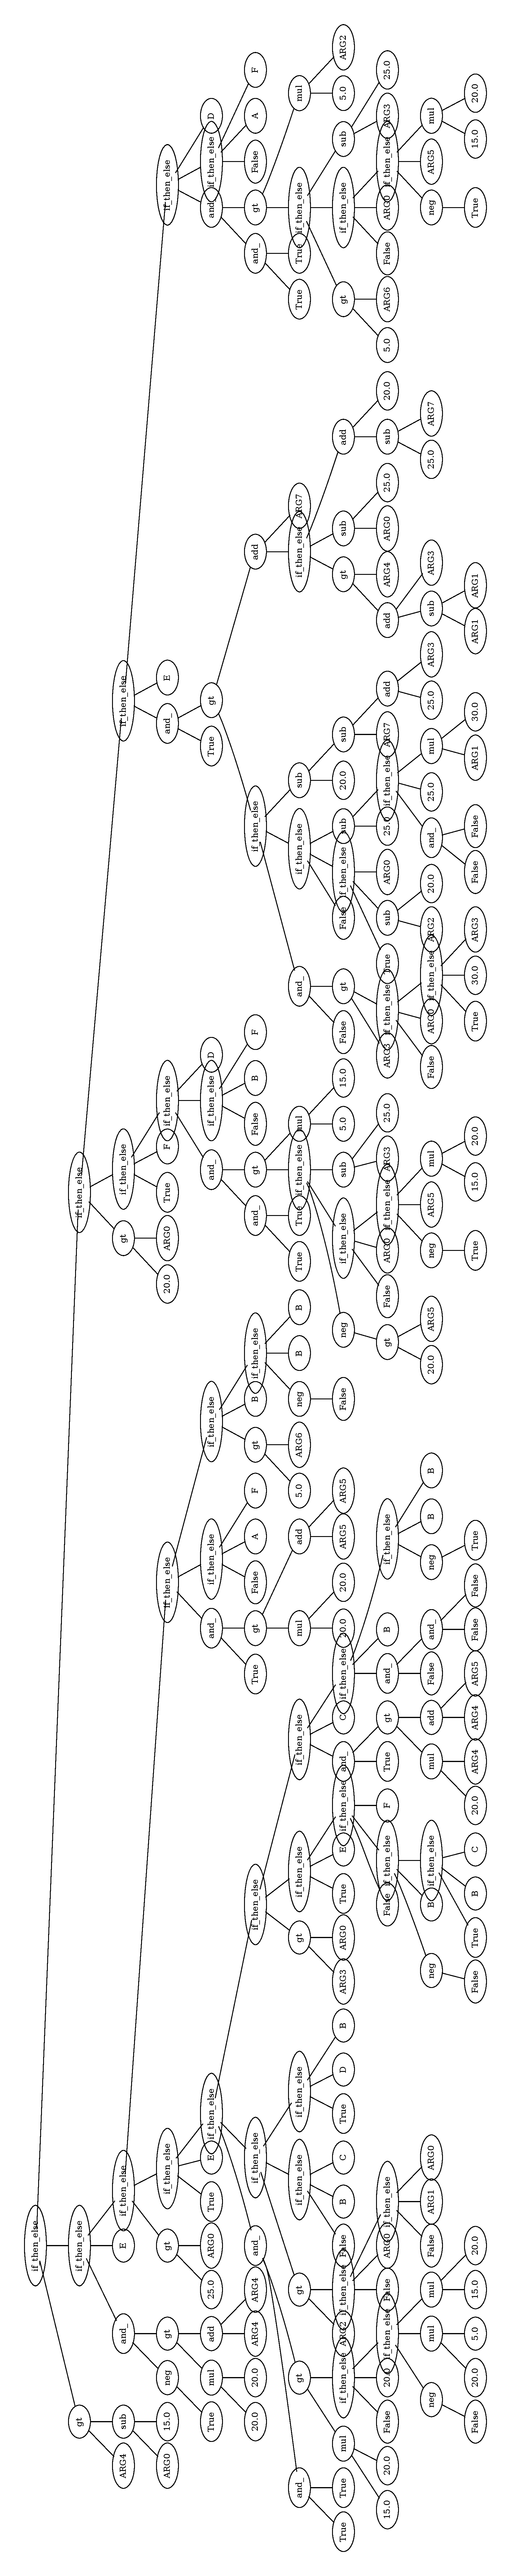
\includegraphics[scale=0.155]{GP_best1.pdf}
        \caption{}
        \label{fig:GP_best1}
    \end{subfigure}
    \hspace{1mm}
    \begin{subfigure}[b]{0.45\textwidth}
        \centering
        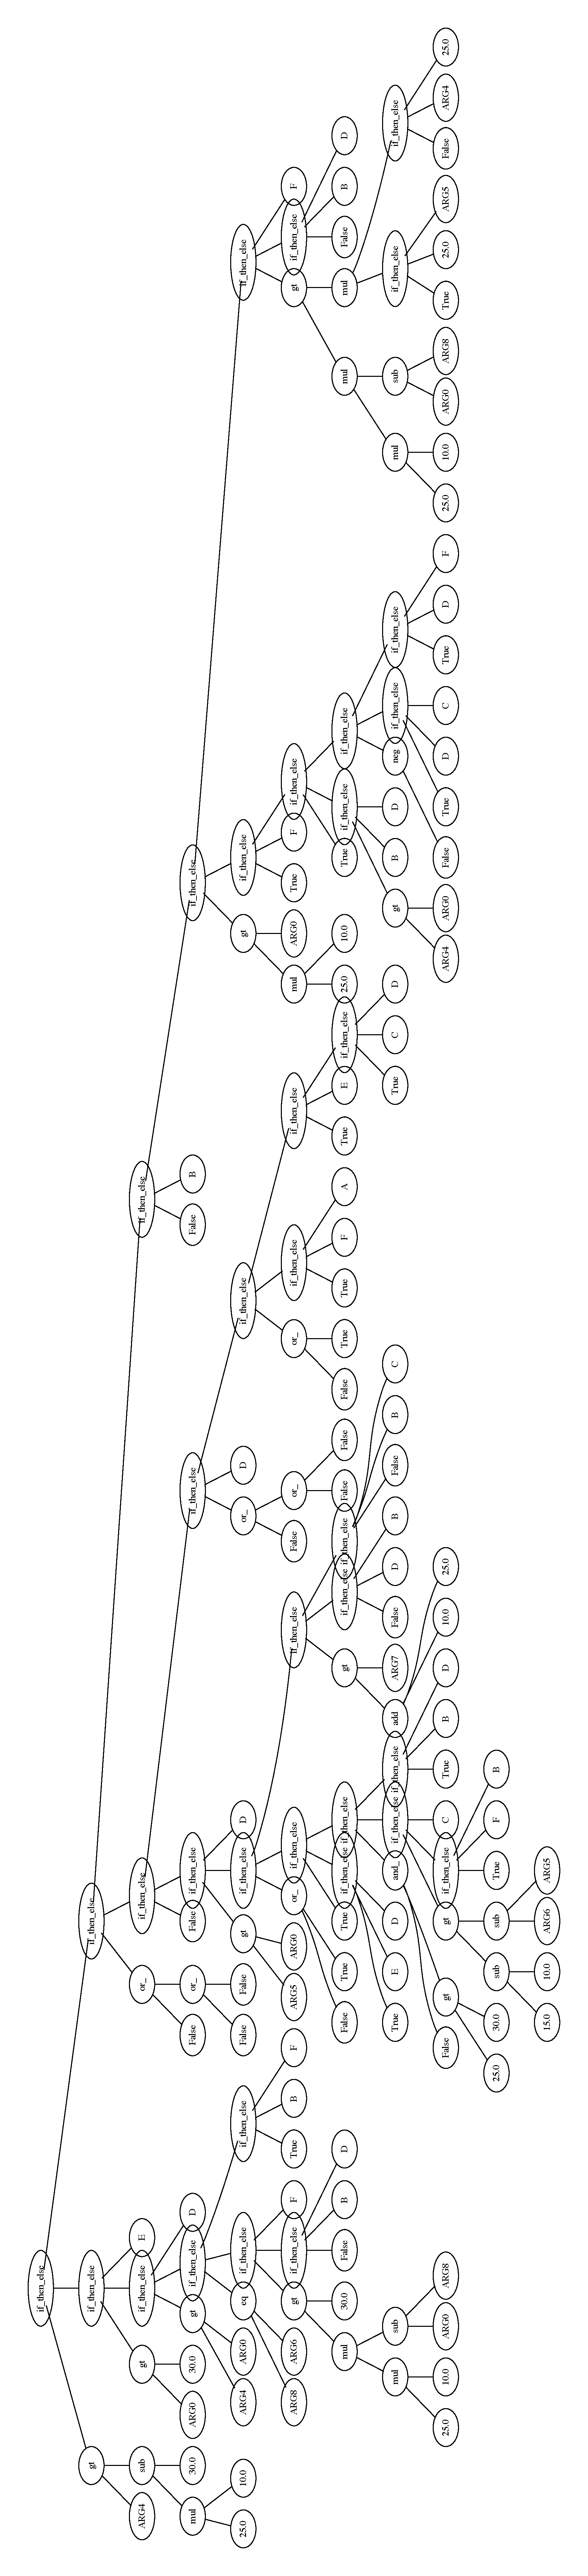
\includegraphics[scale=0.155]{GP_best2.pdf}
        \caption{}
        \label{fig:GP_best2}
    \end{subfigure}
       \caption{Best tree-based programs generated by GP.}
       \label{fig:GP_best}
\end{figure*}


\begin{figure*}[t!]
    \centering
    \begin{subfigure}[b]{0.45\textwidth}
        \centerline{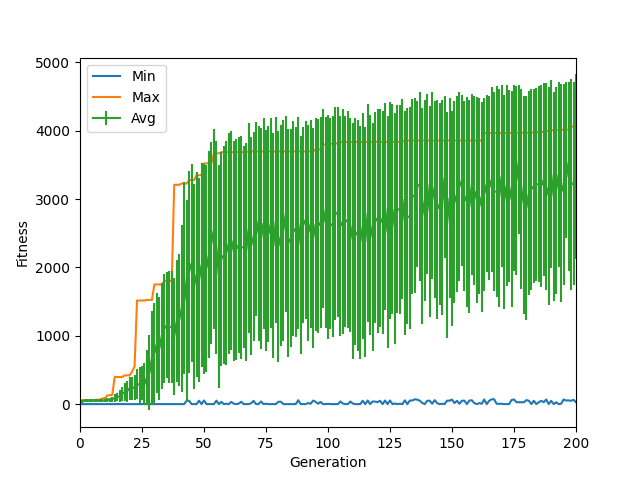
\includegraphics[scale=0.6]{GP_fitness1.png}}
        \caption{}
        \label{fig:GP_fitness1}
    \end{subfigure}
    \hfill
    \begin{subfigure}[b]{0.45\textwidth}
        \centerline{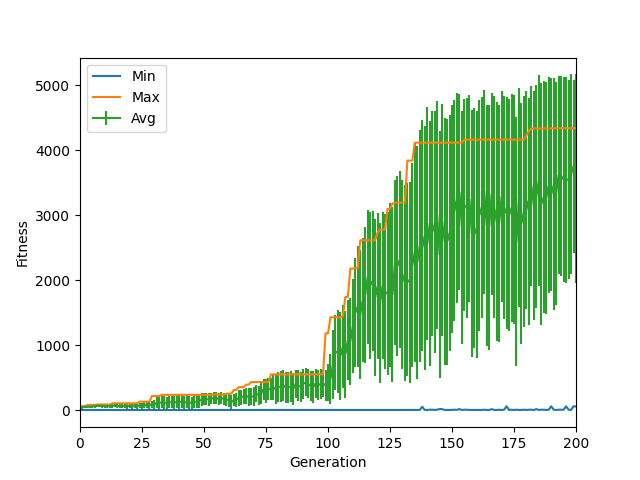
\includegraphics[scale=0.6]{GP_fitness2.png}}
        \caption{}
        \label{fig:GP_fitness2}
    \end{subfigure}
       \caption{Fitness trend of the GP runs that have generated the best programs.}
       \label{fig:GP_fitness}
\end{figure*}

\subsection{Comparison}
With both techniques, we managed to find a program that is able to play the game well,
learning to fire almost always to hit enemies while dodging their lasers.

Considering our scenario, GP demonstrated to have a bigger potential: thanks to the
tree-structure and the functions provided, it is able to learn more complex strategies
reaching level 194, much more than the best evolved ANN. NEAT, instead, struggles to
evolve the network reaching at most level 42. NEAT is probably more suitable for
tasks where a program would not be the best option or even it would be impossible
to build.

Moreover, a tree with a limited size can be more interpretable than a ANN and we can easily
provide an explanation for what the agent is doing.

Observing the agent in action we can say that both NEAT and GP agents move quite smoother, even though
neither of them resemble humans. GP agent, in the end, looks smarter and tends 
to stay in the middle of the playing area dodging all the lasers, whereas NEAT tends to
remain in the corners.

Across multiple runs, NEAT seems to obtain more stable results with respect to GP that 
manages to reach very good results only few times, as shown in Fig. \ref{fig:boxplots}. Both the techniques
find a program which performs much better than a randomly piloted battleship that on average is able 
to reach only level 3 with a fitness of about 45 as shown in Fig. \ref{fig:random_boxplot}.


\begin{figure*}
    \centering
    \begin{subfigure}[b]{0.3\textwidth}
        \centering
        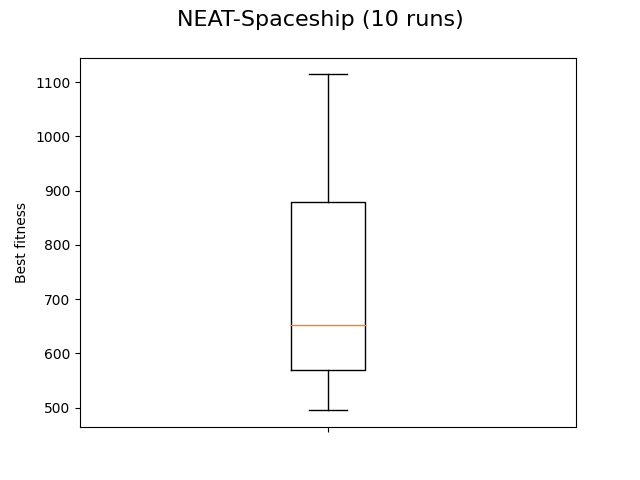
\includegraphics[scale=0.365]{NEAT_Boxplot.png}
        \caption{NEAT boxplot.}
    \end{subfigure}
    \hspace{3mm}
    \begin{subfigure}[b]{0.3\textwidth}
        \centering
        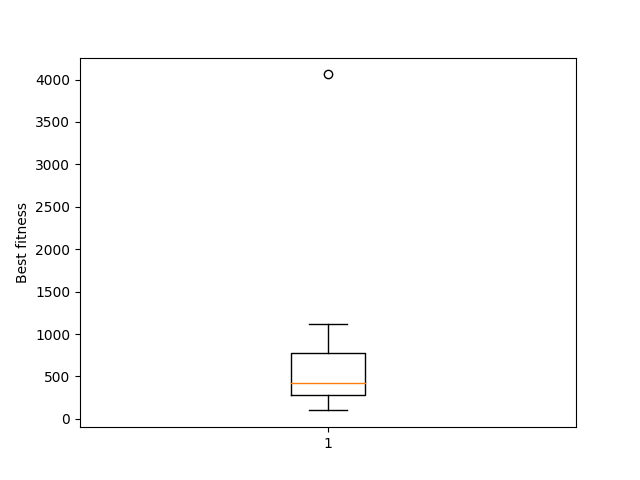
\includegraphics[scale=0.365]{GP_Boxplot.png}
        \caption{GP boxplot.}
    \end{subfigure}
    \hspace{3mm}
    \begin{subfigure}[b]{0.3\textwidth}
        \centering
        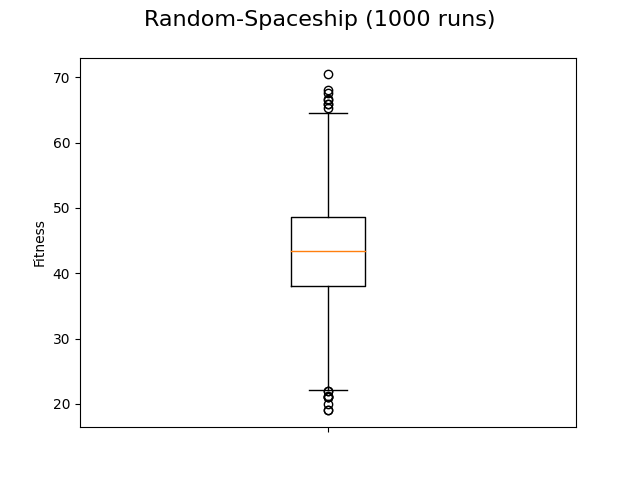
\includegraphics[scale=0.365]{Random_Boxplot.png}
        \caption{Random-piloted battleships boxplot.}
        \label{fig:random_boxplot}
    \end{subfigure}
       \caption{Comparison between the boxplots of NEAT, GP, and randomly piloted battleships.}
       \label{fig:boxplots}
\end{figure*}\
